\documentclass{conference}

% Packages
\usepackage{graphicx}

% Begin document
\begin{document}
{\center \Large \bfseries \MakeUppercase{Using traffic analysis to identify Tor} \par}

{ \center
  \begin{tabular*}{\textwidth}{cccc}
  John Barker & Peter Hannay & Christopher Bolan & Patryk Szewczyk \\
  jebarker@our.ecu.edu.au & p.hannay@ecu.edu.a & c.bolan@ecu.edu.au & p.szewczyk@ecu.edu.au \\
  \end{tabular*}
}

\begin{abstract}

Traditional attacks against anonymous systems aim to uncover the identities of those involved. However, a more likely goal of attackers is to block or degrade the network itself, discouraging participation and forcing vulnerable users to communicate using less secure means. Since anonymous networks operate on known protocols and employ strong encryption it is difficult to distinguish them from regular traffic. This proposal describes a method for identifying traffic belonging to anonymous networks by examining their communication patterns.

\end{abstract}

\section{Introduction}

The Internet has revolutionised the political sphere in providing a platform for the publication of speech to a far greater audience than was ever available before digital communications systems \citep{Bonchek:1997p3455}. The publication of less desirable political speech, criticism or challenging ideas still carries with it great risk, with numerous publications leading to arrest. This has spawned headlines such as \emph{Egypt arrests another blog critic} \citeyear{website:egypt-arrests}, \emph{Chinese couple sue Yahoo! in US over torture case} \citep{website:china-yahoo-torture}, \emph{Vietnam bloggers arrested over China shirt protest} \citep{website:vietnam-bloggers-arrested}, \emph{23 Journalists/Bloggers Arrested in Iran, Including Head of Top Group} \citeyear{website:iran-bloggers-arrested} and \emph{Blogger Arrests} \citep{website:blogger-arrests}. The Internet, like conventional media is still vulnerable to censorship by oppressive governments and malicious attackers \citep{Crandall:2007p6165,Karlin:2009p6166}.

In response to these threats, a number of systems have been proposed which use cryptography to provide censorship resistance and anonymity, including The Second Generation Onion Router (Tor). Tor is an anonymous network which uses various techniques to provide low latency anonymity to network participants \citep{Dingledine:2004p314}. It also aims to provide resistance against censorship based blocking attempts \citep{Dingledine:2008p1542}.

Although Tor provides censorship resistance and a certain amount of privacy, it may be possible to use traffic analysis techniques to automatically identify Tor connections and target them for attacks. Since Tor relies on large numbers of users for the protections it provides, attacks that affect the reliability of the network can discourage participation, rendering it`s protections useless. This paper proposes a statistical methodology for identifying Tor traffic which may be used for such attacks in the future.

\section{Significance}

Tor`s availability, unrestrictive license and platform portability has made it a popular anonymous network with around one thousand eight hundred users at the time of writing \citep{website:tor-anonymity-online}. It has been the subject of many technical papers proposing traffic analysis attacks, however the primary objective has historically been attacks that reveal the identity of participants. As stated in \citet{Murdoch:2005p325} ``The principal objective of an adversary attacking an anonymous communication system is to link the initiators of connections with their respective communication partners and vice versa''.

The traffic analysis techniques proposed in this paper will attempt to classify network streams belonging to Tor users and distinguish them from regular encrypted communications.

\section{Research Questions}

The ability of Tor to connect on any port and it`s usage of strong encryption mean that recognizing traffic belonging to Tor is not straightforward. However it is possible that the communications patterns exhibited by Tor nodes are recognizeable using statistical methods.

This raises the question: is it possible to distinguish the traffic created by these networks, from encrypted traffic produced by conventional software? This question can be broken down further:

\begin{enumerate*}
\item Can the traffic be classified using automated matching techniques?
\item Do these networks have characteristics that make them readily distinguishable using heuristics based matching?
\item Do they have characteristics that make them distinguishable using a machine learning technique?
\item How long does a user have to be connected to the network before a confident match can be made?
\end{enumerate*}

\section{Background Information}

The first anonymous network system was proposed in \citet{Chaum:1981p296}. This proposal included the use of public key cryptography and a centrally located server known as a `mix'. By wrapping the information and address of a destination in a message and encrypting it with the mix`s public key, only the mix system is able to read the message.

\subsection{The Second Generation Onion Router (Tor)}

The Tor network, like the Mix-Net proposed by \citet{Chaum:1981p296} uses public key encryption and cascades of servers to ensure message anonymity \citep{Dingledine:2004p314}. In Tor these mixes are known as ‘relays’. Relays that allow connections directly from Tor clients are known as ‘bridges’ and relays that deliver messages from the frontier of the Tor network are known as ‘exit nodes’. Figure \ref{tor-network} shows how a client connects to the Tor network.

\begin{figure}[H]
\center 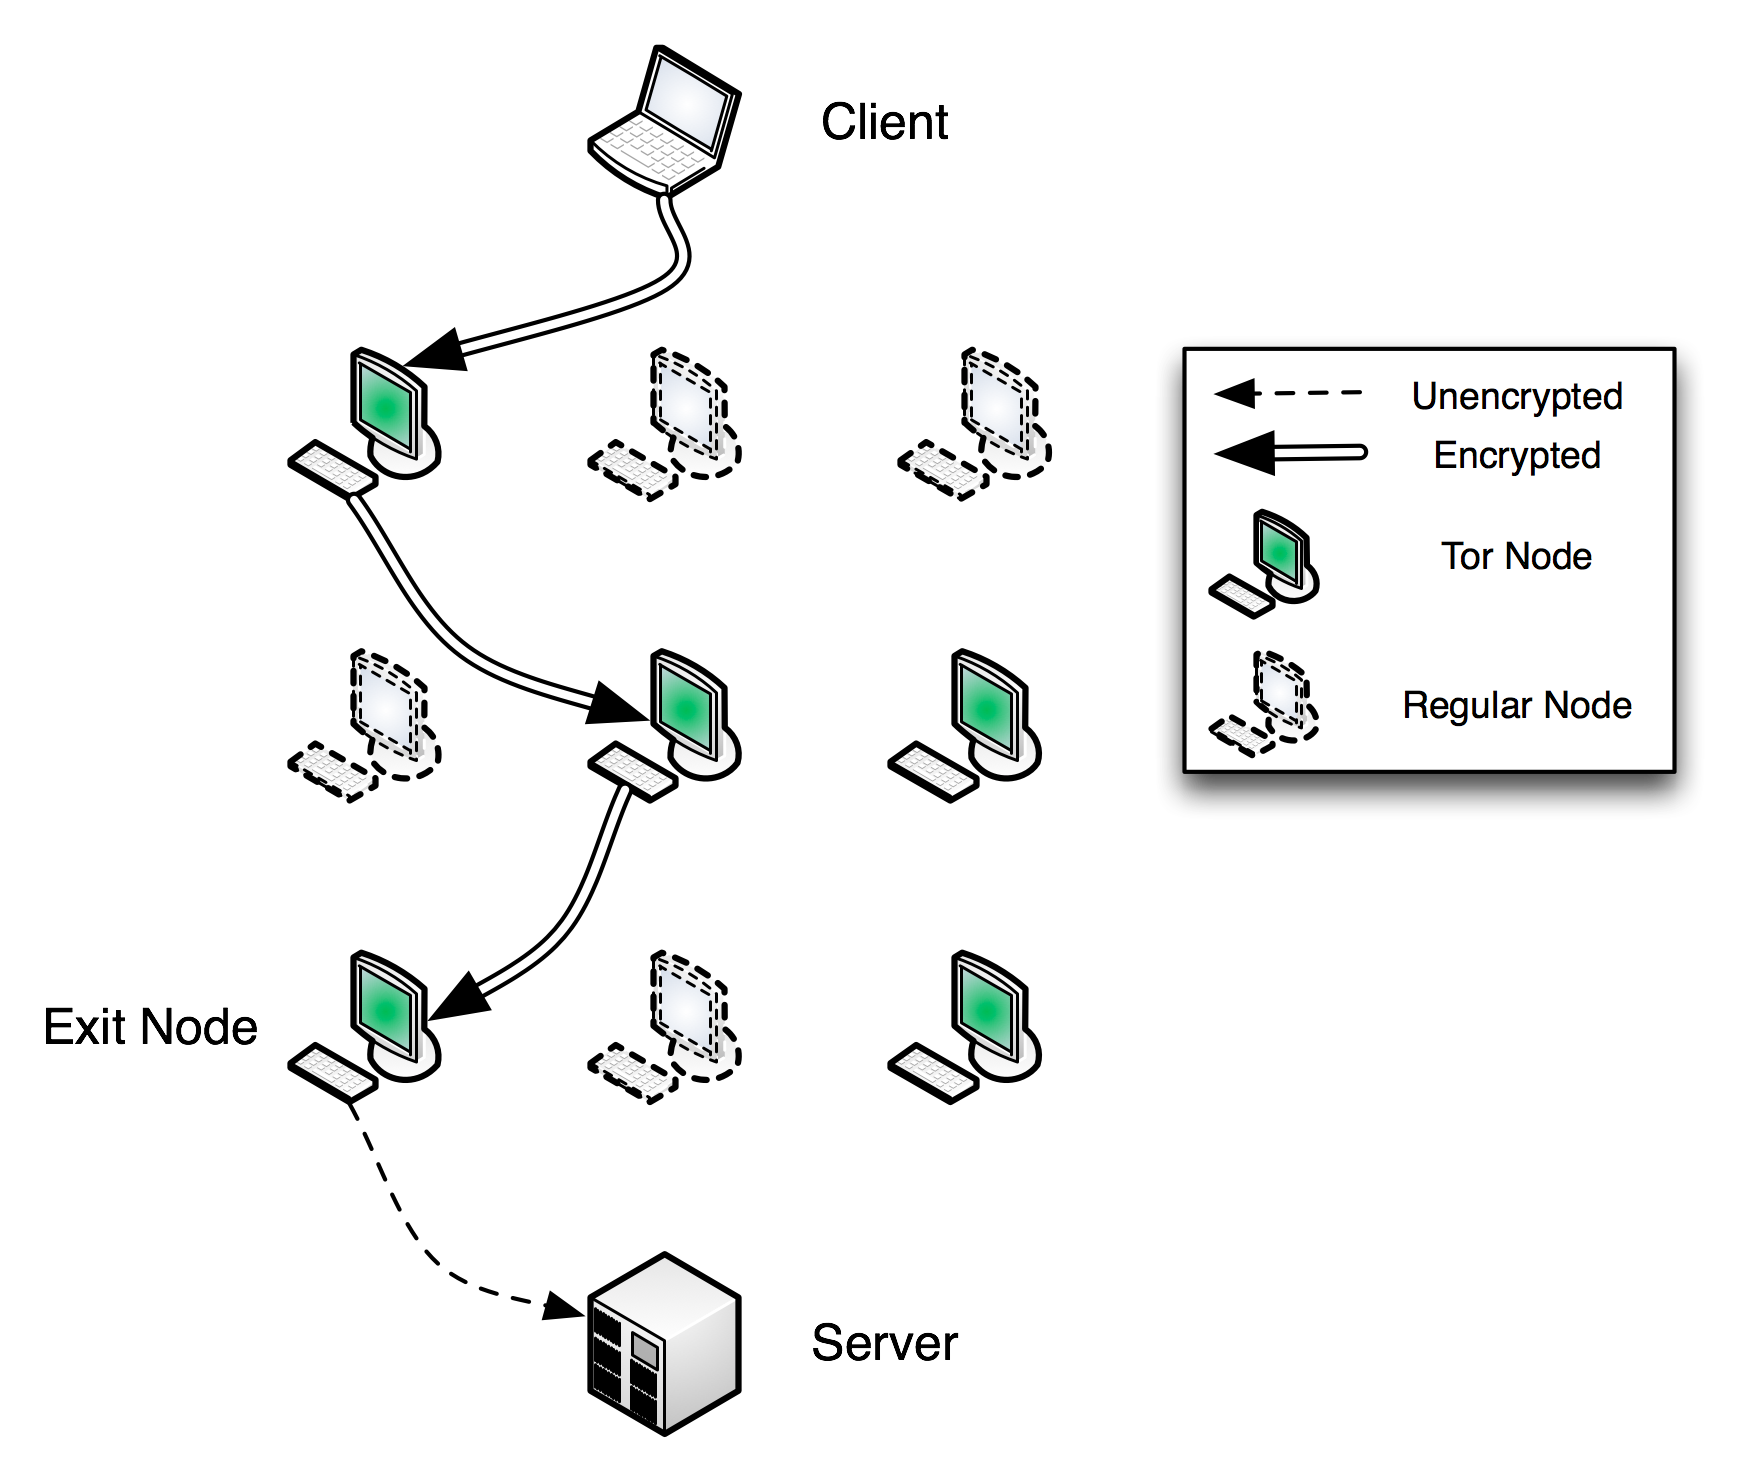
\includegraphics{tor-network-diagram}
\caption{The Tor Network}
\label{tor-network}
\end{figure}

When a relay joins the Tor network, it trades symmetric cipher keys with its neighbours using public key cryptography. These keys are used to encrypt communications and are destroyed when the session is closed to prevent replay attacks.

After it was noticed that Tor was being used to circumvent censorship as well as for anonymity, a proposal was developed to improve its blocking resistance \citep{Dingledine:2008p1542}. Many of the suggestions in this proposal have been implemented, but many still remain.

\section{Related Work}

When considering the use of traffic analysis for Internet communications, three primary techniques are used. These are: exact matching, heuristic matching and machine learning \citep{Zhang:2009p1188}. Exact matching techniques are ineffective in recognizing Tor communications as Tor can operate on any available port and uses encryption to hide communications. This leaves heuristic and machine learning matching techniques.

\subsection{Heuristic Techniques}

The increasing burden of peer to peer (P2P) applications on campus networks, and their shift to encryption motivated the development of heuristics based techniques for identifying P2P traffic. Early techniques include identifying known properties of P2P networks such as often communicating using both the UDP and TCP protocols simultaneously and using a solitary connection to transfer high volumes \citep{Karagiannis:2004p6400}. Similar techniques have been developed in \citep{Perenyi:2006p6325} and \citep{John:2008p1376}, both of which attempt to improve matching accuracy by expanding the scope of matching parameters and eliminating false positives using exact matching techniques.

Heuristics based matching techniques have also been used to identify traffic belonging to network worms \citep{Lazarevic:2003p6450} and the Skype protocol \citep{Ehlert:2006p2396}.

\subsection{Machine Learning Techniques}

\subsubsection{Expectation-Maximisation}

The first use of machine learning to categorise traffic flows appears in \cite{McGregor:2004p3826}. A detailed analysis of the attributes that can be used for machine learning and an attempt at coarse grained classification using an Expectation-Maximisation (EM) algorithm are demonstrated. The same technique is also demonstrated in \cite{Soule:2004p3817} using histograms for finer grained classification. The EM algorithm is again used in \cite{Zander:2005p6212} and \cite{Erman:2006p3825}, with the latter also comparing this algorithm favourably against a Naïve Bayes classifier.

\subsubsection{Naïve Bayes}

\cite{Moore:2005p3827} use a supervised Naïve Bayes to classify traffic flows that have previously been sorted into groups by analysing the flow content. This paper focuses on many of the most commonly used Internet protocols while \cite{Bonfiglio:2007p6453} uses the technique for identifying traffic belonging to the commercial Skype application.

\cite{Herrmann:2009p1189} use Bayesian networks to fingerprint visited websites accessed through Privacy Enhancing Technologies (PET), including Tor. This technique performed poorly when applied to the Tor network, but it suggests that Tor traffic has particular characteristics that distinguish it from many existing PETs. It makes a particularly useful observation: “The most frequent packet sizes in the Tor traffic dumps are, in descending order, 1500, −52, −638, 52, 638 and 1150 bytes, accounting for 87.6 \% of all Tor packets.”

\subsubsection{Hidden Markov Model}

Hidden Markov Models are first used as a traffic analysis technique in HMM profiles for network traffic classification \citep{Wright:2004p3860}. The primary identification characteristics for use with this algorithm are packet size and inter-packet arrival times. With refinement this algorithm is used with increasing accuracy in \cite{Wright:2006p322} and \cite{Dainotti:2008p1435}. HMMs are also used in \cite{Bernaille:2005p6205} to discover distinguishing characteristics of traffic flows, rather than specifically as a classifier.

\subsubsection{Clustering}

Clustering algorithms group observations into subsets based on similar characteristics. They have been used in a number of traffic classification techniques with the K-Means clustering technique being the most prominent. K-Means cluster analysis appears in Bernaille et al. (2006), \cite{Erman:2007p3764}, \cite{Erman:2007p6206}. The use of the Density Based Spatial Clustering of Applications with Noise (DBSCAN) algorithm appears in \cite{Erman:2006p3766}, alongside K-Means and Autoscan algorithms.

\subsubsection{Other Techniques}

Other algorithms used for traffic classification include Nearest Neighbour and  Linear Discriminant Analysis \citep{Roughan:2004p3823}, Normalized Threshold \citep{Crotti:2007p3824}. The use of the Gaussian Mixture Model to identify applications and identities inside SSH tunnels was demonstrated in \cite{Dusi:2008p6254}.

\subsubsection{Comparing Techniques}

It is difficult to say what machine learning technique is the most effective as no consensus has been reached, the literature covers a wide variety of techniques each with vastly different goals and no two techniques can be directly compared as the data used for analysis has not been disclosed \citep{Kim:2007p3867}. However some attempt has been made at comparison in \cite{Williams:2006p3849} which suggests that the C4.5 algorithm has the greatest performance and accuracy when compared to a number of Bayesian algorithms. \cite{Mohd:2009p6484} compares thirty machine learning algorithms  to find random tree, IBI, IBK and random forest algorithms obtaining the greatest classification accuracy.

An excellent meta study on traffic analysis techniques is presented in \cite{Nguyen:2008p3837}. This paper compares many of the published papers, the techniques used, criteria analysed and how effectively they meet stated goals.

\section{Theoretical Framework}

The proposed research will use a methodology typical of machine learning traffic analysis papers, substituting data captured from a controlled simulation in place of live network captures. 

The experiment will be conducted in two phases, the first being a data collection phase. The second phase will include a quasi experimental methodology which may include data manipulation techniques to prepare the collected data and a comparison of various heuristics and machine learning based traffic analysis to classify the collected data.

\subsection{Assumptions}

It is assumed that the usage patterns exhibited by individual users will be smaller than the communications characteristics that will lead to the identification of anonymous and censorship resistant networks. Thus there is no need to obtain a large sample of regular network traffic from varying user profiles.

As of the current implementation, Tor network traffic is readily distinguishable by looking at the handshake packets. It is likely that this weakness will be addressed in a future version of the Tor protocol as it is recognised as a design goal in \cite{Dingledine:2008p1542}. For this reason, this proposal focuses on traffic analysis techniques that are content agnostic.

\subsection{Variables}

The data capturing stage will be affected by a number of variables that will influence the accuracy of the chosen matching algorithms. These include:

\begin{enumerate*}
\item System Performance
\item Network Performance
\item Application Protocol
\item Quality of the Anonymous Network
\item Caching
\end{enumerate*}

An attempt will be made to reduce the impact of these variables by capturing packets generated by an isolated simulation of the Tor network, ensuring only vital network applications are running and executing software inside a virtual machine which can be rolled back to a known snapshot \citep{website:snapshot-definition}.

\section{Materials and Methods}

The experiment will consist of two phases, first a simulation phase which involves the capture of packets belonging to a Tor network

Figure \ref{network-diagram} shows the placement of applications and relevant data flows.

\begin{figure}
\center 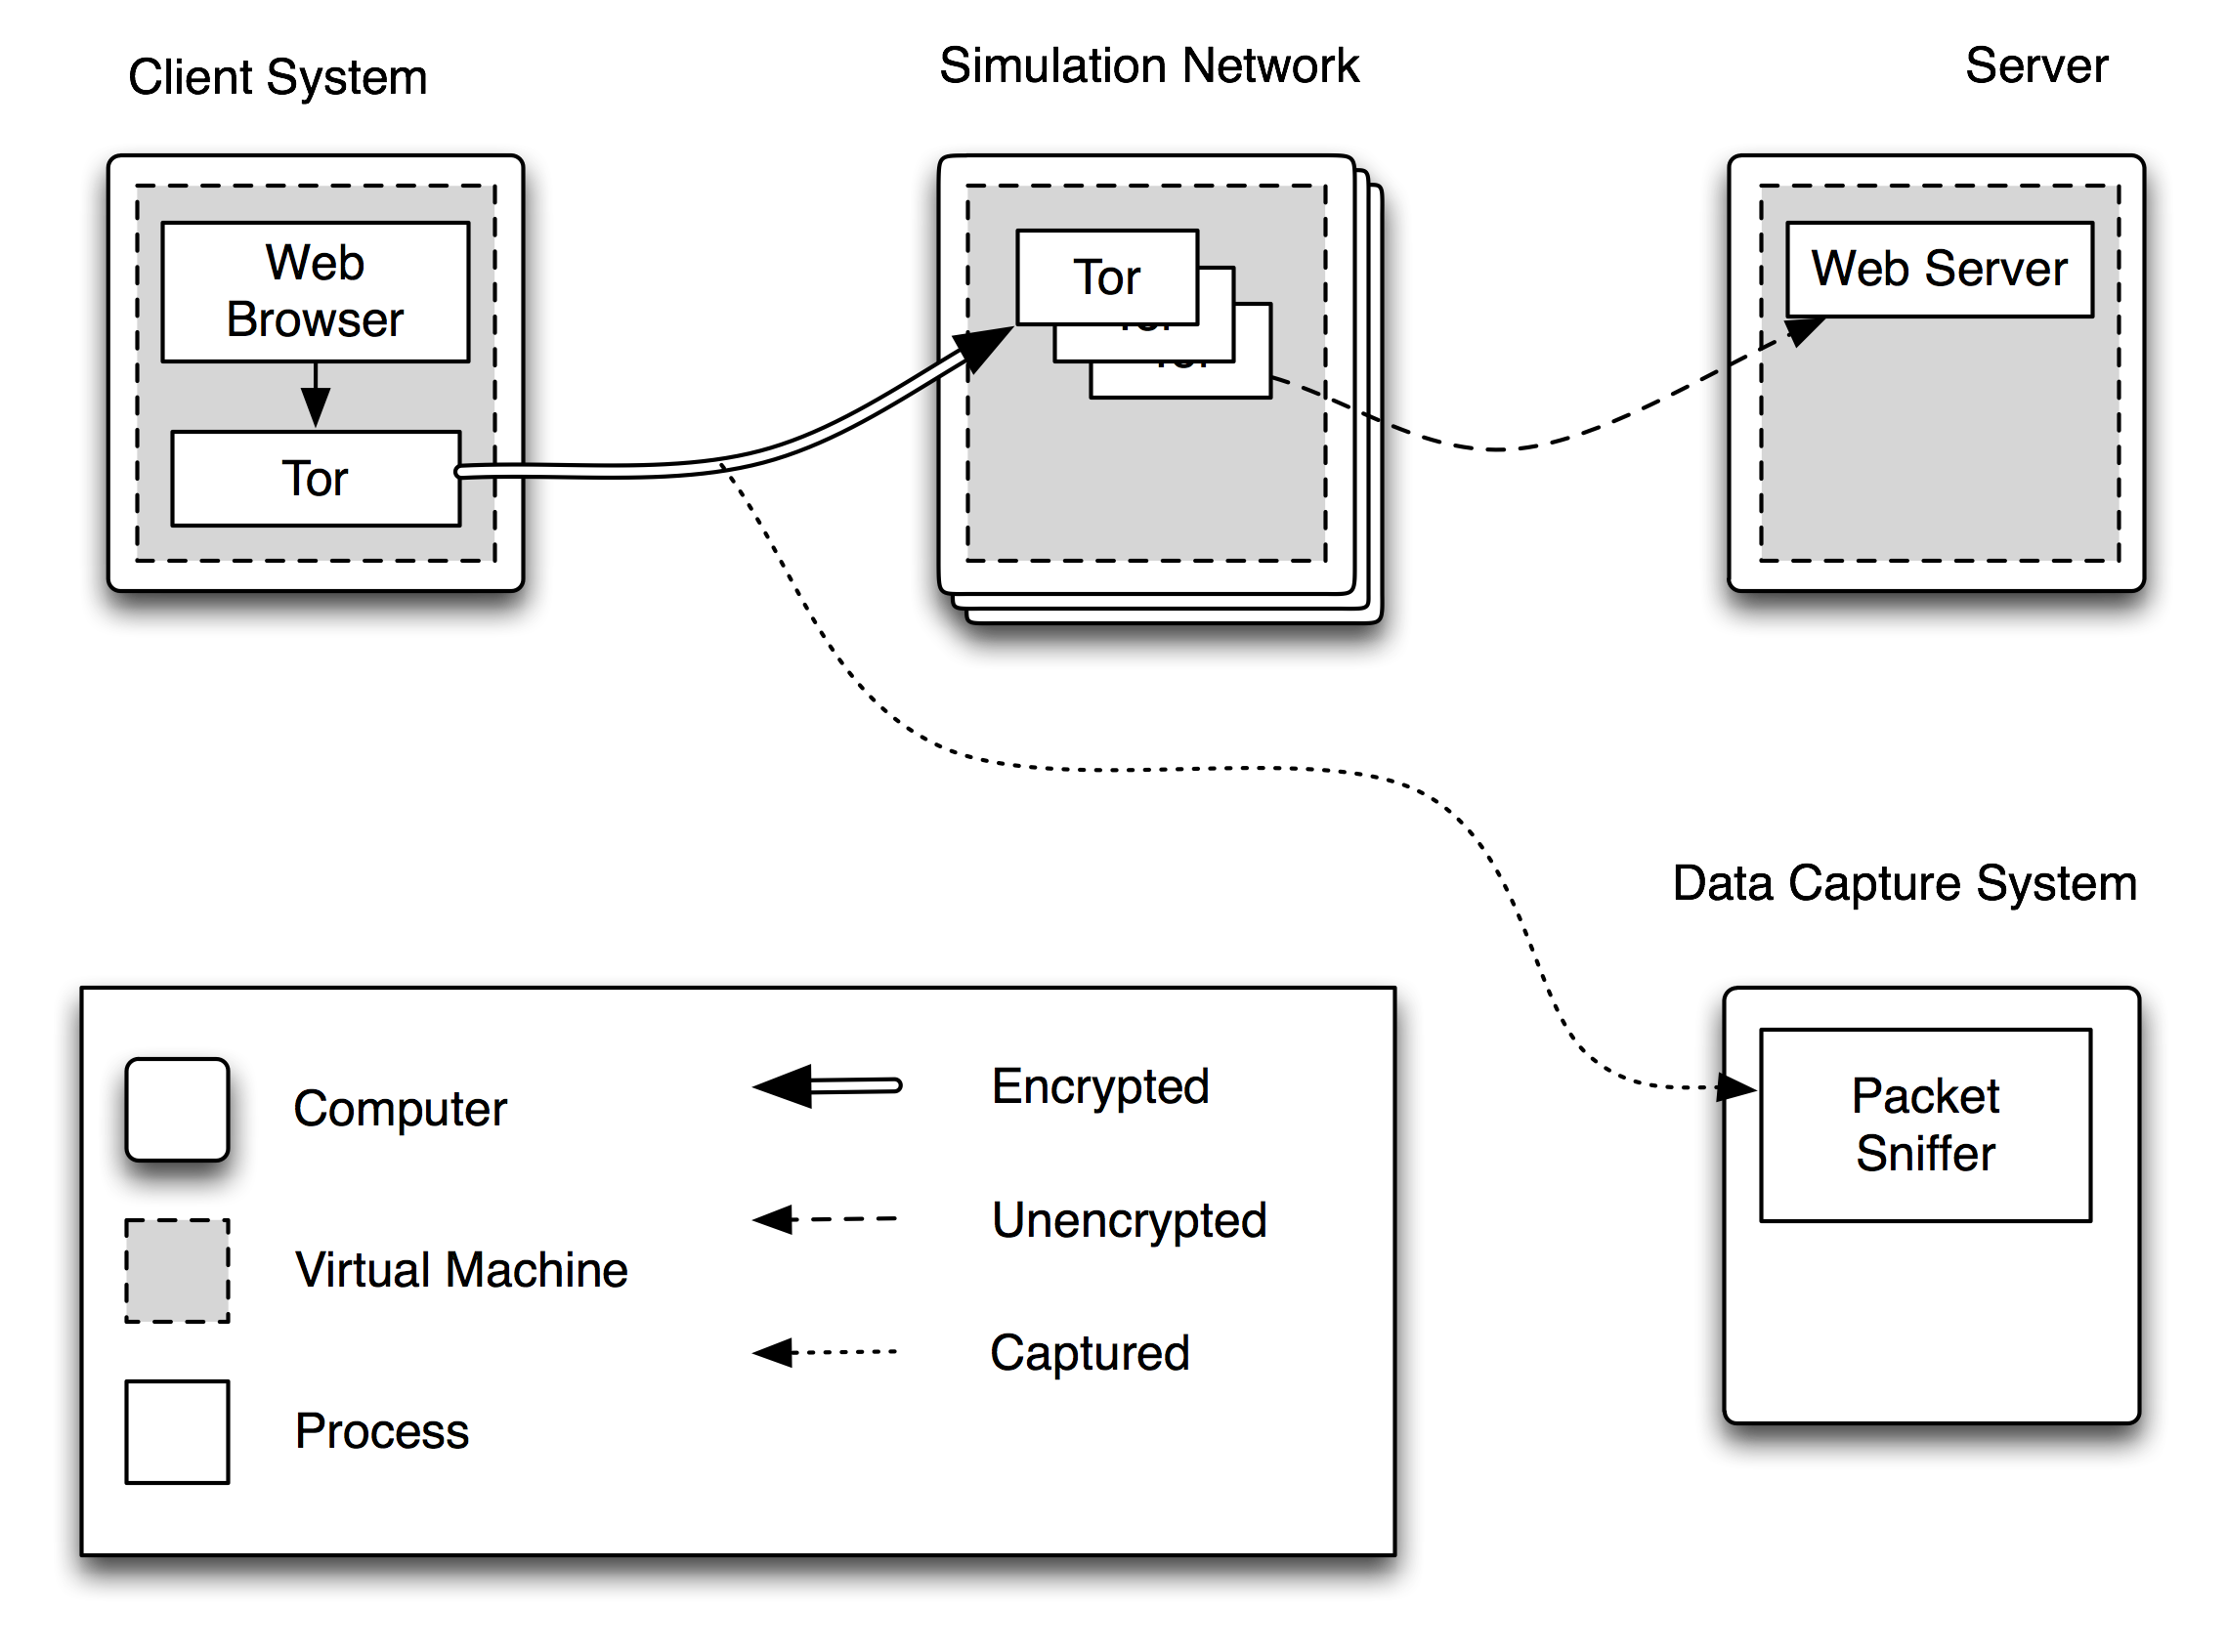
\includegraphics[scale=0.8]{network-diagram}
\caption{Network Diagram}
\label{network-diagram}
\end{figure}

\bibliography{papers,websites}

\end{document}

% vim: fdm=syntax
